% This version of CVPR template is provided by Ming-Ming Cheng.
% Please leave an issue if you found a bug:
% https://github.com/MCG-NKU/CVPR_Template.

%\documentclass[review]{cvpr}
\documentclass[final]{cvpr}

\usepackage{times}
\usepackage{epsfig}
\usepackage{graphicx}
\usepackage{amsmath}
\usepackage{amssymb}

% Include other packages here, before hyperref.

% If you comment hyperref and then uncomment it, you should delete
% egpaper.aux before re-running latex.  (Or just hit 'q' on the first latex
% run, let it finish, and you should be clear).
\usepackage[pagebackref=true,breaklinks=true,colorlinks,bookmarks=false]{hyperref}


\def\cvprPaperID{****} % *** Enter the CVPR Paper ID here
\def\confYear{CVPR 2021}
%\setcounter{page}{4321} % For final version only


\begin{document}

%%%%%%%%% TITLE
\title{Exploring Conditional Invertible Neural Networks \\}

\author{
Final Project for the course Computer Vision: 3D Reconstruction\\\\
Damjan Kalšan, Scientific Computing, 3707396\\
David Scheid,  Data \& Computer Science, 3666910\\
Sebastian Stricker, Scientific Computing, 3677266\\
Heidelberg University, WS2021/22\\
}

\maketitle


%%%%%%%%% ABSTRACT
\begin{abstract}
   In the following we document our experiments with the conditional invertible neural network (cINN) architecture as proposed by \cite{main_paper_CINN}.
   In the first part, the concept is illustrated on a simple toy example to provide a more intuitive understanding of the image generation and style transfer process.
   The second part focuses on the application on new data. We chose FashionMNIST \cite{fashion_mnist} as a simple yet diverse dataset and show results and difficulties with image generation and style transfer.
   We build our models using the FrEIA framework \cite{freia}
\end{abstract}

%%%%%%%%% BODY TEXT
\section{Introduction}
In usual classification tasks with neural networks, a network is trained to predict a class label, a one hot encoded vector $y$, given an input vector $x$. This can be represented as $f(x; \theta) = y$, with $\theta$ being the network weights.

In contrast to this, cINNs are provided with this information by a conditioning vector $c$ during the forward pass already. The resulting output or latent vector $z$ necessarily matches the input in dimension to preserve invertibility of the network. Figure \ref{fig:cINN_concept} illustrates the concept.

This key property of invertibility allows for the inverse mapping  $z \rightarrow x$. Equation \ref{eq:cINN} captures this. It is achieved by constructing the network as a concatenation of coupling blocks as introduced by \cite{RealNVP}.
For the technical details, we refer to the original publications.

\begin{equation} \label{eq:cINN}
\begin{split}
		f(x;c;\theta) 		= z \\
		f^{-1}(z;c;\theta) 	= x
\end{split}
\end{equation}

For the models discussed in this work $c$ can be seen as equivalent to the ground truth one-hot encoding $y$. As demonstrated by more complex image coloration architectures \cite{main_paper_CINN}, the conditioning can also take other forms, however.

\begin{figure}[t]
	\begin{center}
		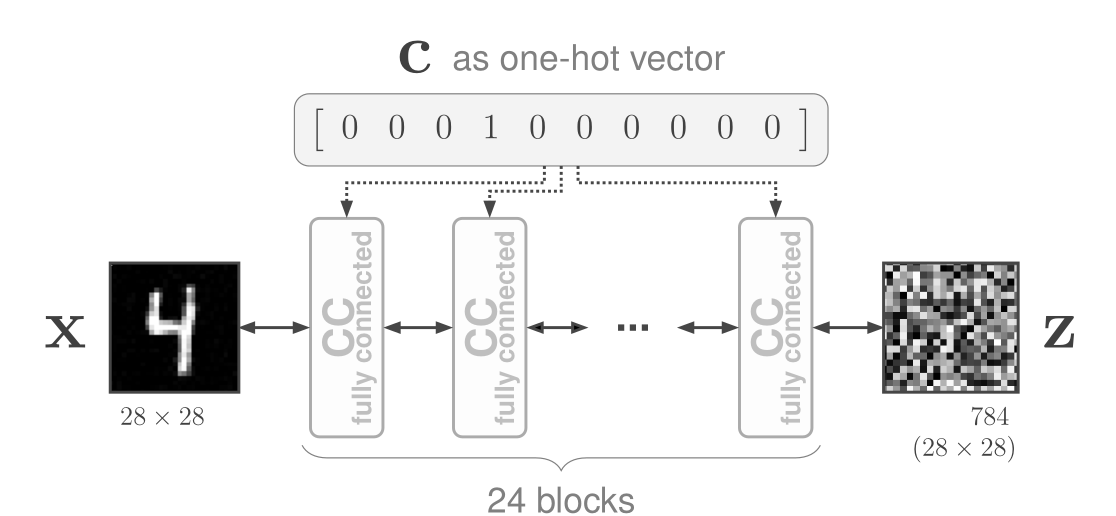
\includegraphics[width=0.8\linewidth]{./figs/cINN_MNIST_model.png}
	\end{center}
	\caption{Illustration of cINN Architecture for MNIST digit classification. Class labels are concatenated to the intermediate input in each coupling layer. Taken from \cite{main_paper_CINN}}
	\label{fig:cINN_concept}
\end{figure}

\subsection{Interpreting the latent vector}
In contrast to classification networks, the output $z$ of cINNs is not trained against a given ground truth. Rather, the agreement between $f$ and $f^{-1}$ is trained. It raises the question of what information $z$ is supposed to contain.

Assume for training data $X$, $Z = \{f(x_i;c;\theta) \,|\, x_i \in X\}$ is the set of all $z$ that are an output of the network. The training enforces $Z$ to take the form of a probability distribution $p_Z(z)$. For simplicity, we assume it to be the standard normal. The training Loss is then a maximum likelihood calculation, meaning the inverse pass should assign $x$ a high probability, given a $z$ and $c$. The weights are adjusted to increase this likelihood $P(X|Z)$.

For technical details, we again refer to the original publication \cite{main_paper_CINN}. \\

As will be shown in section \ref{toy}, interpreting the individual dimensions in the latent space is not trivial. But seen as a whole, $z$ has to capture all the features that make up our input in order to ensure the map $z \rightarrow x $ holds, while maintaining the property that the complete set $Z$ forms the given probability distribution. 

\subsection{Image generation and style transfer}
$Z$ is a finite set, but the probability distribution enforced on the set is a continuous function. Therefore, it is possible to sample from the distribution to obtain a $z' \notin Z$. Running the network in reverse results in $f^{-1}(z';c;\theta) = x'$. $x'$ is then a result, that has not been generated before. 

For style transfer, a $z$ is obtained from an arbitrary $x$ via the network $f(x;c_x;\theta) = z$. Setting $c' \neq c_x$, the style of $x$ can be mapped to all other class labels via $f(z;c';\theta)$.

\section{Toy example}\label{toy}
In the following, a simple example using 4 gaussian distributions is used to illustrate and explore properties of the cINN mappings described in the Introduction.

The model used consists of 8 AllInOne coupling blocks, described in the framework \cite{freia}. As a subnet for each block, a fully connected network with 2 hidden layers and 256 nodes each is employed.

\begin{figure*}[t]
	\begin{center}
		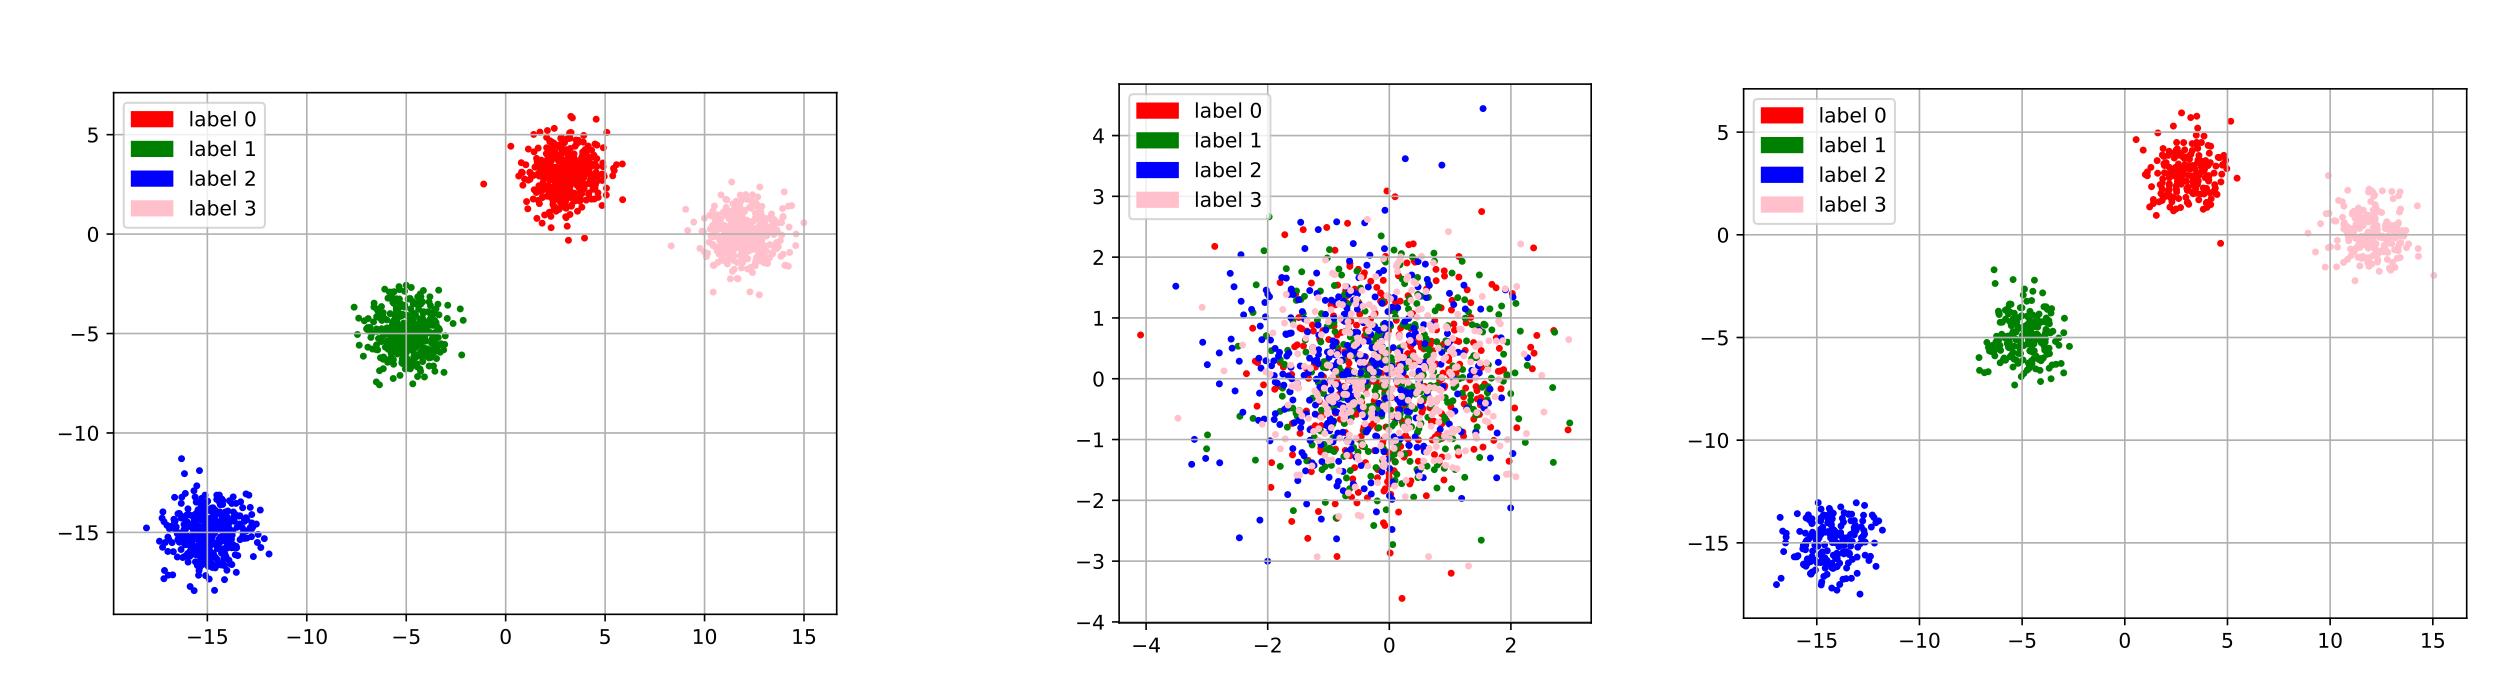
\includegraphics[width=1.0\linewidth]{./figs/toy/no_style/combined.png}
	\end{center}
	\caption{(left) Input data. (middle) Latent space after training. (right) Data generated with newly sampled z values.}
	\label{fig:toy_generation}
\end{figure*}

\subsection{Sample Generation}\label{sec:toy_sample}
Figure \ref{fig:toy_generation} depicts the process of image generation. 

The left plot shows the input data. Each distribution contains 800 samples. Labels used for conditioning indicate which distribution a point originates from and are color coded in the plots to visually differentiate between them.
Positions of samples form the respective input vector $x = (\hat{x}, \hat{y})$

The middle image depicts the latent space $Z$ after training. Visibly, the values form a normal distribution as enforced by training. Further, the values are not separated by label. Clearly no classification information is stored in the latent space.

The right image depicts the result of data generation. For each label, 200 values from a two dimensional normal distribution were drawn and passed through the inverse network.
As can be seen, the data was successfully classified even though the $z$ values used were not part of the training process.

\subsection{Style transfer}
To make matters more interesting, each sample was enhanced with an attribute from the set $S = \{0.0, 1.0, 2.0\}$. The input vector is then formed by $x = (\hat{x}, \hat{y}, s)$, with $s \in S$ chosen randomly for each sample.

After training, 5 samples from label 0 distribution were evaluated resulting in $Z'=\{z_1, z_2, z_3, z_4, z_5\}$. For all labels, these $z$ samples were then passed through the inverse network. 
The results are depicted in Figure \ref{fig:toy_style}. The plot to the left shows the input distributions and the one to the right the results after style transfer. 
Attribute value s is indicated by shape and was rounded to the nearest integer after the inverse pass.

As can be seen, the samples with label 1,2,3 have successfully received the shapes from the samples with label 0. This result was consistent over many attempts. 

Position transfer, on the other hand, does not seem to work consistently. In the example depicted here, apart from small deviations, samples in label 0 and 1 seem to have been assigned equivalent positions. Samples in label 2 and 3 have been rotated counterclockwise by 90°.
Depending on training success and chance, results on position transfer range from fully consistent to not correlated at all.

\begin{figure*}[t]
	\begin{center}
		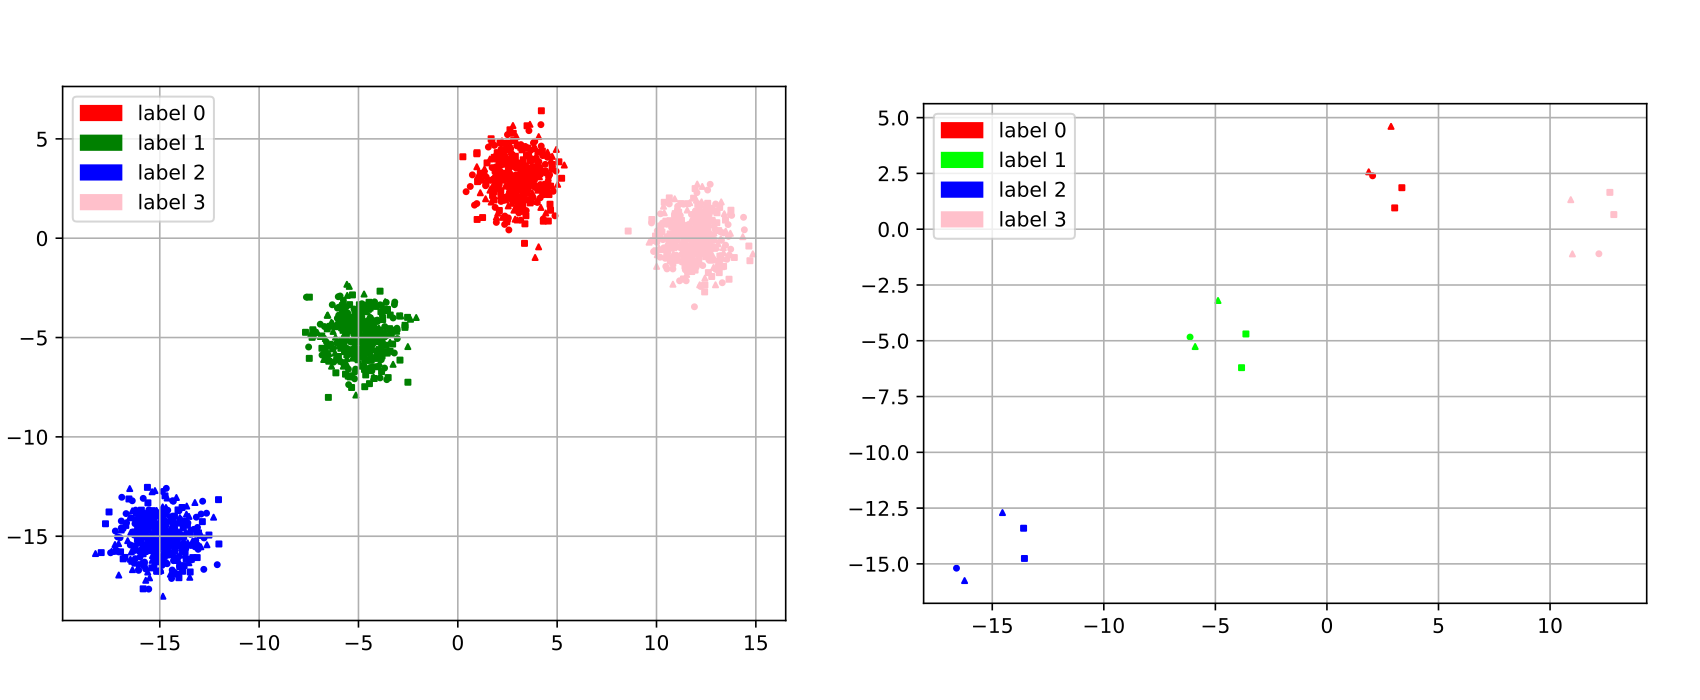
\includegraphics[width=1.0\linewidth]{./figs/toy/with_style/combined_style_transfer.png}
	\end{center}
	\caption{(left) Input data. Attribute $s$ is plotted as corresponding shape \{circle, square, triangle\} (right) Successful style transfer of label 0 to all labels.}
	\label{fig:toy_style}
\end{figure*}

\subsection{Attribute enhanced latent space}
To close the section on the toy example, it is shown that dimensions in the latent space do not necessarily capture information independent from each other. 

Similar to the sample generation as described in section \ref{sec:toy_sample}, 200 $z$ vectors were sampled from the three dimensional normal distribution.
Dimensions were then searched for correlation with attribute information $s$. The corresponding dimension differs for each training run. 

In the network analysed, the second dimension contained the highest degree of information. For each sample a constant value $c$ replaced the corresponding value $z = (z^1, z^2, z^3) \rightarrow (z^1, c, z^3)$.

Figure \ref{fig:latent} shows the results for $c = \{-2.0, 0.0, 2.0\}$. As can be observed, the samples do all receive the same attribute, however, the positions are in no example as clear as in the initial distributions.
It can be concluded, that the latent space dimensions are not easily separable in this example.

\begin{figure*}[t]
	\begin{center}
		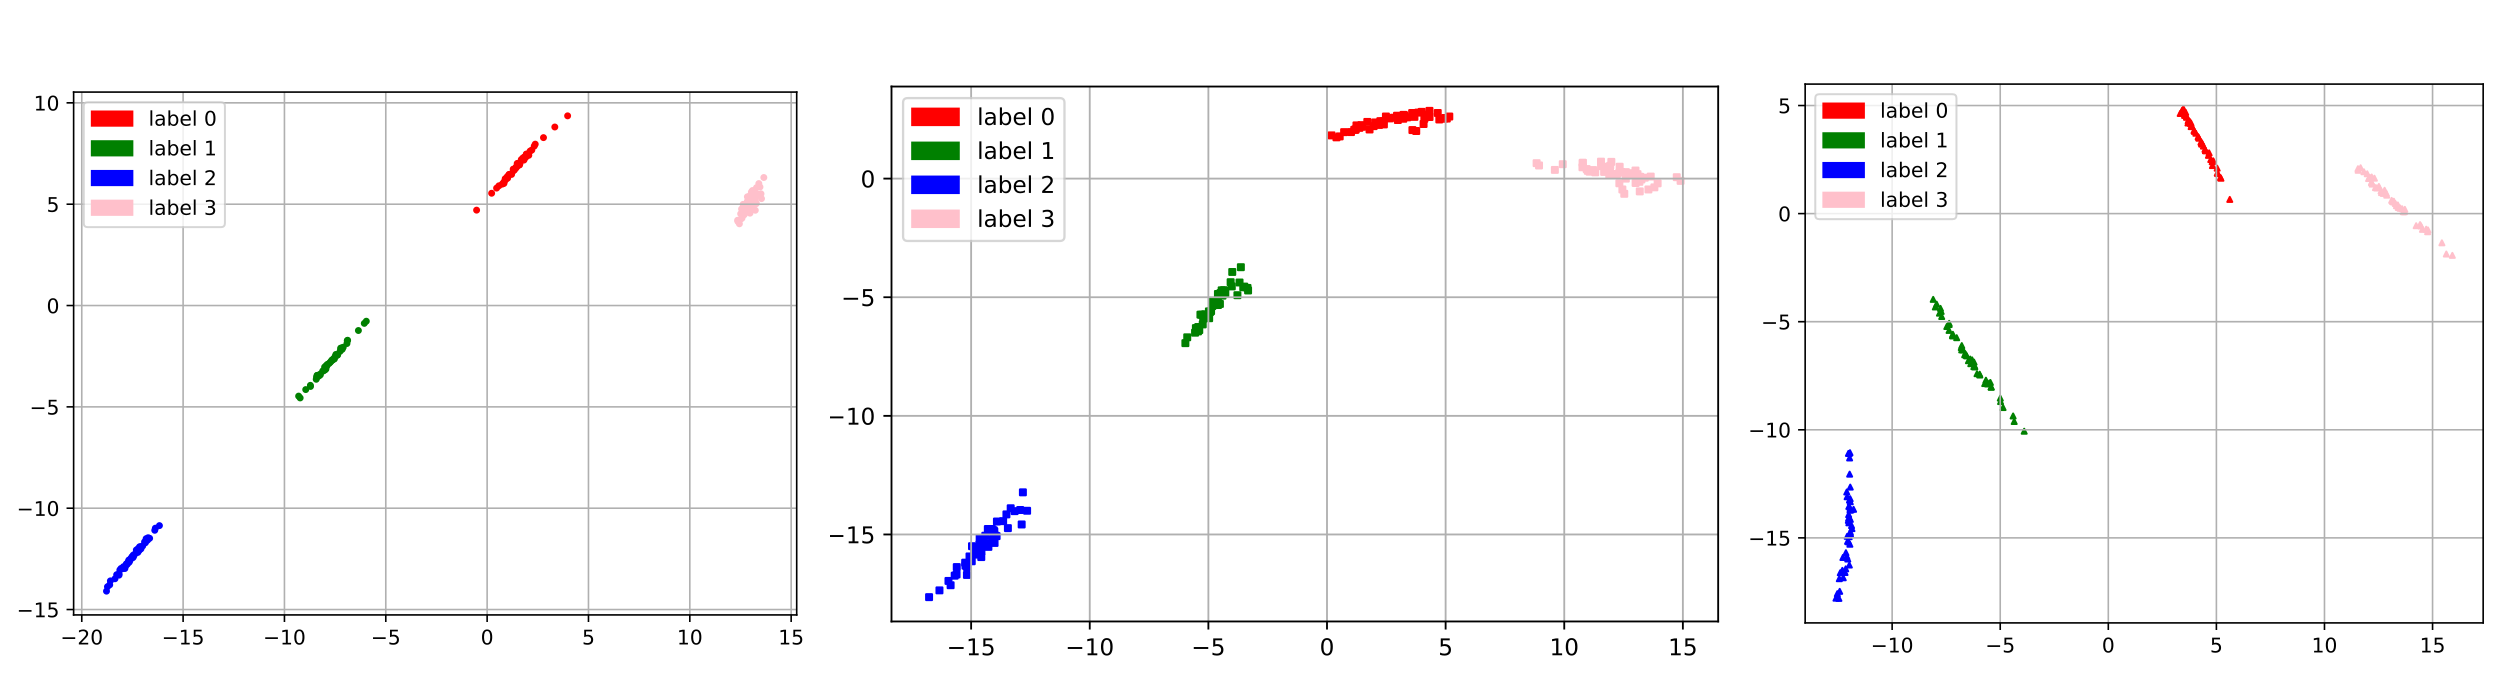
\includegraphics[width=1.0\linewidth]{./figs/toy/with_style/combined_reverse_sample.png}
	\end{center}
	\caption{(left) $c = -2.0 \Rightarrow s = 0.0$ (circle). (middle) $c = 0.0 \Rightarrow s = 1.0$ (square). (right) $c = 2.0 \Rightarrow s = 2.0$ (circle).}
	\label{fig:latent}
\end{figure*}

\section{Application to FashionMNIST}
In this section we applied cINNs to the FashionMNIST dataset. Considering that the latter is meant to serve as a direct drop-in replacement for the MNIST dataset \cite{fashion_mnist}, we chose a simple architecture design illustrated in Figure \ref{fig:cINN_concept} as our baseline. We then tried to improve this architecture through performing 4 main experiments and documented the main findings. 

\subsection{Sample generation}
All explored architectures use the GLOW coupling blocks, first introduced in \cite{GLOW}, in combination with a fixed random permutation along the channel dimension. Moreover, we augment the training data with noise sampled from a Gaussian distribution.  The exception is experiment in Subsection \ref{sec:experiment_softflow}, where we opt for a specialized augmentation procedure.

\subsubsection{Baseline}\label{sec:experiment_baseline}
As a subnet within each coupling block we used a fully connected network with a single hidden layer of 512 nodes, followed by a ReLU activation. Such subnets are also employed in all subsequent experiments.

We find that the samples generated by this architecture lack details. Namely, they do not contain any patterns such as stripes or checkerboards, but rather only generate the rough shape of the conditioned item, commonly of a homogeneous color. This is not the case for sandals, which often consist of thin lines and cannot be reproduced by the network. For the most part, the correct item is generated as per conditioning, however there is still a small portion of outliers. This is the case for items, which are visually similar, such as pullover and coat. Moreover we notice that some of generated dresses have a darker vertical gap in the middle and effectively look like something in between a dress and trousers. Lastly the network sometimes generates white noisy blobs instead of the conditioned item. All aforementioned shortcomings are addressed in successive experiments and can be observed in Figure \ref{fig:fashionmnist_baseline_samples}.

\begin{figure}[t]
	\begin{center}
		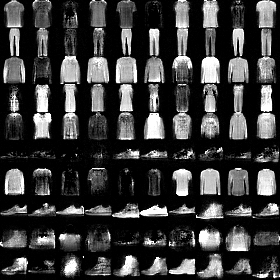
\includegraphics[width=0.8\linewidth]{./figs/fashion_mnist/baseline_model_samples.png}
	\end{center}
	\caption{Samples generated with the baseline model described in \ref{sec:experiment_baseline}. Starting from the top, conditioned classes are: t-shirt/top, trouser, pullover, dress, coat, sandal, shirt, sneaker, bag, ankle boot.}
	\label{fig:fashionmnist_baseline_samples}
\end{figure}


\subsubsection{Convolutional network with FCN conditioning}
In this experiment we prepended the baseline architecture with convolutional coupling blocks and reduced the number of fully-connected ones to 15. Specifically we consider our architecture in four stages, where we gradually downsample the image using Haar wavelets, as proposed in \cite{main_paper_CINN}, and increase the hidden channels of our convolutional layers. At the end of each stage we create a skip connection to the latent space, halving the channels dimension. The first stage consists of 5 coupling blocks operating on the original image, which we duplicate along the channel dimension. This is needed, because we are working with grayscale images and the coupling blocks split the input to two parts. The second stage works on a downsampled output of the first, using 5 convolutional coupling blocks. Analogously the third stage works on the downsampled output of the second, employing 10 convolutional coupling blocks. Lastly, we flatten the output of the third layer and feed it into the fully-connected coupling blocks. Imporantly, in this experiment we condition only on the last stage, as our labels come in form of a one-hot encoding.

Generally the new architecture outperforms the baseline, as it produces sharper lines on the item borders and the items better resemble their corresponding shapes. There are still no good patterns, but there seems to be an attempt at doing so. Namely on some items, such as t-shirts, we noticed artifacts which appear more like noise than a consistent pattern. Moreover on the chest part of t-shirts we observe holes of different color than the item itself. We assume this corresponds to prints which are common in the training data for this item. The network is capable of reproducing sandals, however in some samples they are still hard to distinguish. Another improvement is that we do not observe white blobs anymore.

We conclude that the convolutional coupling blocks are crucial for quality reconstruction and stick to the introduced four-stage architecture in the following experiments.

\subsubsection{Conditioning on all coupling blocks}\label{sec:experiment_condition_on_all_ccs}
In hopes to reduce outliers based on conditioned class, we extended the conditioning information to the convolutional coupling blocks. Each block received a one-hot encoded feature map conditioning of corresponding image height and width, with values from set $C = \{\frac{1}{10}, \frac{2}{10}, ..., \frac{10}{10}\}$, where the numerator represents class label incremented by one. This proved to give equal results to having ten separate feature maps, one for each class, at a reduced computational cost.

Upon inspection of generated samples, we concluded that the quality did not increase enough to stand out and that the percentage of outliers stayed essentially the same. Nonetheless, we kept this conditioning for the remainder of experiments. Some generated samples can be seen on Figure \ref{fig:fashionmnist_final_model_samples}.

\begin{figure}[t]
	\begin{center}
		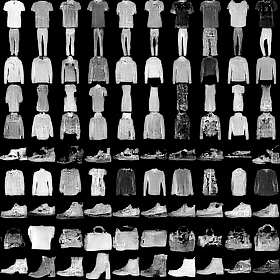
\includegraphics[width=0.8\linewidth]{./figs/fashion_mnist/final_model_samples.png}
	\end{center}
	\caption{Samples generated with the experimental model described in \ref{sec:experiment_condition_on_all_ccs}. Starting from the top, conditioned classes are: t-shirt/top, trouser, pullover, dress, coat, sandal, shirt, sneaker, bag, ankle boot.}
	\label{fig:fashionmnist_final_model_samples}
\end{figure}

\subsubsection{Removing skip connections}
Skip connections generally help with fine detail reconstruction, as the latter can be lost through repeated convolution operations. Hence we removed them from the model to assess their importance in our architecture.

As expected, the network had trouble generating finer details in some items, such as bags and sandals. We also observed some noisy samples with unrecognizable shape. The quality of the rest of the items did not change.

\subsubsection{SoftFlow}\label{sec:experiment_softflow}
In cases where the training data distribution sits on a lower-dimensional manifold, current flow-based models perform poorly in terms of sample generation \cite{softflow}. Employing SoftFlow, a solution proposed in \cite{softflow}, models can effectively learn to better reconstruct details, an open issue with our current approach. We assessed this by adding perturbations to our training data, specifically, each image was augmented with Gaussian noise of uniformly sampled standard deviation $\sigma \in [0.01, 0.10]$. The latter was then appended to the conditioning next to the class. For convolutional coupling blocks, we added a feature map filled with $\sigma$, while for the fully-connected coupling blocks we simply added $\sigma$ at the end of one-hot-encoded vector.

This augmentation procedure failed to produce favorable results in our case. The generated samples are more diverse in color, ranging from nearly invisible black colored samples to light gray. In contrast, the previous augmentation procedure yields extremely bright samples to the point of saturation with darker colors being less common, yet still present. We notice however a degraded quality in generation of sandals, where thin lines in some samples disappear. Changing the interval of sampled standard deviations $\sigma$ also did not result in better generated samples. Not only that, but with $\sigma \in [0.1, 0.2]$ we found noise around the surface of generated samples.

\subsection{Style transfer}
...

\section{Conclusion}
In the first part we explored conditional invertible neural networks on a toy example, giving intuition behind the latent space, as well as performed sample generation and style transfer. In the second part we applied them to a new dataset and explored different architectures. We found that sample generation is challenging even for a simple dataset like FashionMNIST. Throughout experimentation we failed to find a model which could generate samples with fine details. In future work, we would be interested in deepening the subnets by adding a second hidden layer. Moreover reducing the number of coupling blocks in the first stage might allow the skip connection to transfer more detailed pixel information to the latent space.

{\small
\bibliographystyle{ieee_fullname}
\bibliography{bibliography}
}

\end{document}
